\begin{quote}
	\glqq Was man an Kraft spart, muss man an Weg zulegen.\grqq
\end{quote}

\noindent Diese einfache Regel bezieht sich auf jegliche mechanische Vorgänge bei denen Körper bewegt werden. Wenn man weniger Kraft aufwenden möchte, muss man den Körper über eine längere Strecke bewegen. 

Das einfachste Beispiel ist das heben eines Körpers. Dieser kann direkt hochgehoben werden, was eine Kraft erfordert, die größer ist, als die Kraft, die die Schwerkraft auf den Körper ausübt. Beispielsweise könnte der Körper aber auch über ein Rampe geschoben werden, welche dann den Weg, über welchen eine Kraft angewendet werden muss, vergrößert, aber die Kraft verkleinert. 

Wenn die Kraft $F$ ist und $s$ der Weg über welchen sie angewendet wird, gilt:

\begin{align}
	F_{1} \cdot s_1 = F_{2} \cdot s_2
\end{align}

\noindent Dies folgt direkt aus der Definition der Energie und dem Energieerhaltungssatz, da $E=F \cdot s$ (Siehe \referenz{sec:energien}).

\subsection{Flaschenzug}

Der Flaschenzug eignet sich sehr gut um diese Beziehung zu zeigen. Man betrachte folgende Abbildung\footnote{„Four pulleys“ von User:Prolineserver, User:Tomia. (minor edits by Stanisław Skowron, scale adjusted by User:Atropos235) - Eigenes Werk. Lizenziert unter CC BY 2.5 über Wikimedia Commons - \url{https://commons.wikimedia.org/wiki/File:Four_pulleys.svg}}:

\begin{figure}[h!]
	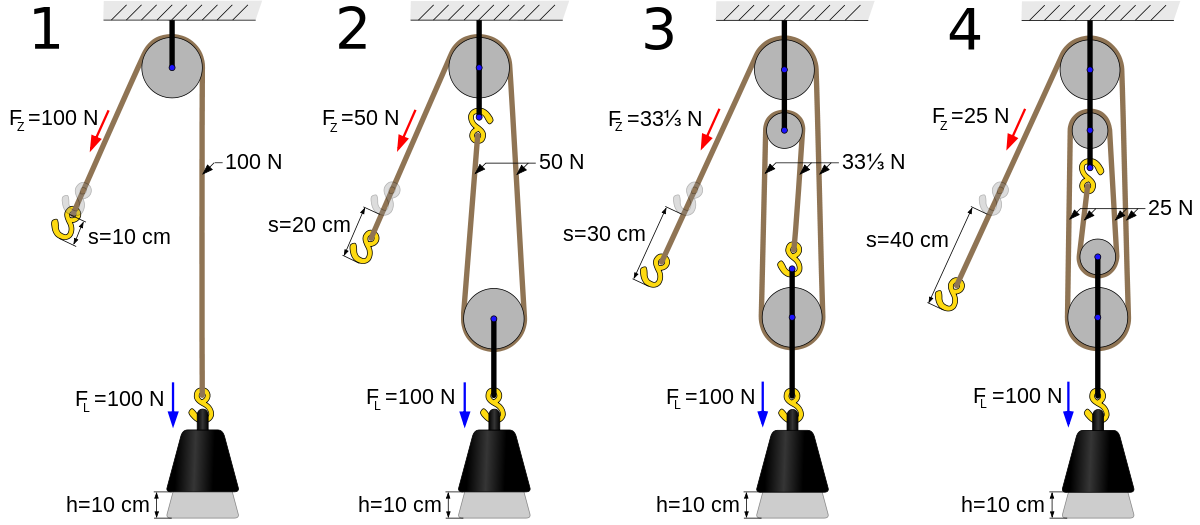
\includegraphics[width=\textwidth]{flaschenzug}
	\caption{4 Flaschenzüge, die dieselbe Last heben}
	\label{fig:flaschenzug}
\end{figure}

Die Last, die eine Gewichtskraft von $100N$ aufbringt, wird jedes Mal um $10cm$ angehoben, das heißt, dass die jeweilige Arbeit, die verrichtet wurde, konstant ist ($W = 100N \cdot 0,1m = 10J$).

Allerdings wird beim Addieren einer weiteren Rolle die Zahl der Seilstrecken, an denen quasi gleichzeitig gezogen wird, größer. Dadurch wird die zu ziehende Strecke $s$ proportional größer und die aufzuwendende Kraft $F_Z$ kleiner.

